%%%%%%%%%%%%%%%%%%%%%%%%%%%%%%%%%%%%%%%%%%%%%%%%%%%%%%%%%%%%%%%%%%%%%%%%%%%%
\documentclass{beamer}           % pdfTeX の場合
% 付録をページ数にカウントしない NPC
\usepackage[orientation=portrait,size=a0,scale=1.3]{beamerposter}% whole 指定
\setbeamertemplate{navigation symbols}{} % ナビゲーションを消す

\usepackage[whole]{bxcjkjatype}% whole 指定
\usepackage{algorithm}
\usepackage{tcolorbox}
\usepackage{algorithmic}
%\usepackage{theorem}
\usepackage{amsthm}
\usepackage{amsmath}
\usepackage{bbm}
%\usepackage[dvipdfmx]{graphicx}
\usepackage{graphicx}
\usepackage{overpic}
%\usepackage[absolute,overlay]{textpos}
\usepackage[relative,overlay]{textpos}
%\setbeamertemplate{background}[grid][step=30pt]

\newcommand{\bhrule}{{\color{blue} \hrule}}

\definecolor{nico}{rgb}{1, 0.90, 0.96}
\definecolor{orange}{rgb}{0.95, 0.3, 0.0}
\definecolor{ash}{rgb}{0.2,0.2,0.5}
\definecolor{hoge}{rgb}{0.53,0.28,0.59}
\definecolor{myblue}{rgb}{0.2,0.2,0.7}
\setbeamercolor{mine}{fg=white,bg=blue!70!cyan}
\renewcommand{\alert}[1]{{\color{orange} {#1} }}
\renewcommand{\structure}[1]{{\color{blue!50!cyan} {#1} }}
\tcbset{colframe=myblue,colback=white,boxsep=16px,before skip=-20px,left=30px} % textcolorbox settings

\newcommand{\plus}{{\color{red} +1}}
\newcommand{\minus}{{\color{blue} -1}}

\title{全部分グラフ指示子上の分類森構築に向けて}
\author{北海道大学大学院~修士1年~横山侑政}

%%%%%%%%%%%%%%%%%%%%%%%%%%%%%%%%%%%%%%%%%%%%%%%%%%%%%%%%%%%%%%%%%%%%%%%%%%%

\setbeamercolor{myframetitle}{fg=white,bg=myblue}

\begin{document}
~ \\
\vspace{10px}
\begin{beamercolorbox}[
    wd=\hsize,
    sep=32pt,     % パディング
]{myframetitle}
\begin{center}
	{\Huge \inserttitle} \\
	\medskip
	\medskip
	{\huge \insertauthor} \\
\end{center}
\end{beamercolorbox}

\begin{columns}[T]
	\begin{column}{0.50\hsize}
		\begin{tcolorbox}[title={\Large グラフの教師あり分類問題}]
	\structure{入力}
	クラス($ y = \plus \mbox{~or~} \minus $)の分かる複数のグラフ $N$ 個
	\vspace{20px}

	\begin{textblock*}{0.2\textwidth}(50pt,0pt)
		\begin{center}
			$\plus$ \\
			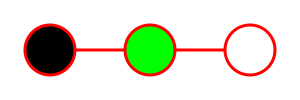
\includegraphics[width=0.6\textwidth]{img/graph/g01r.png}
		\end{center}
	\end{textblock*}

	\begin{textblock*}{0.2\textwidth}(250pt,0pt)
		\begin{center}
			$\plus$ \\
			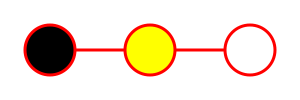
\includegraphics[width=0.6\textwidth]{img/graph/g02r.png}
		\end{center}
	\end{textblock*}

	\begin{textblock*}{0.2\textwidth}(450pt,0pt)
		\begin{center}
			$\plus$ \\
			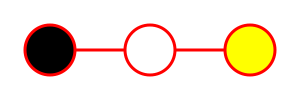
\includegraphics[width=0.6\textwidth]{img/graph/g03r.png}
		\end{center}
	\end{textblock*}

	\begin{textblock*}{0.2\textwidth}(650pt,0pt)
		\begin{center}
			$\minus$ \\
			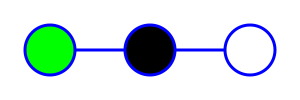
\includegraphics[width=0.6\textwidth]{img/graph/g04b.png}
		\end{center}
	\end{textblock*}

	\begin{textblock*}{0.2\textwidth}(50pt,150pt)
		\begin{center}
			$\minus$ \\
			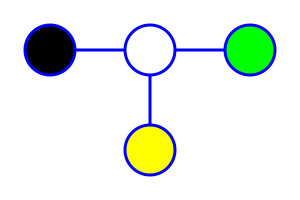
\includegraphics[width=0.6\textwidth]{img/graph/g05b.png}
		\end{center}
	\end{textblock*}

	\begin{textblock*}{0.2\textwidth}(250pt,150pt)
		\begin{center}
			$\minus$ \\
			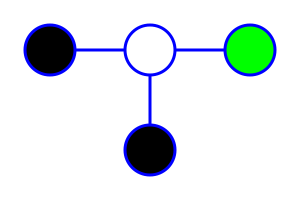
\includegraphics[width=0.6\textwidth]{img/graph/g06b.png}
		\end{center}
	\end{textblock*}

	\begin{textblock*}{0.2\textwidth}(450pt,150pt)
		\begin{center}
			$\plus$ \\
			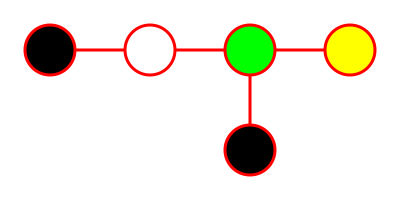
\includegraphics[width=0.6\textwidth]{img/graph/g07r.png}
		\end{center}
	\end{textblock*}

	\begin{textblock*}{0.2\textwidth}(650pt,150pt)
		\begin{center}
			$\minus$ \\
			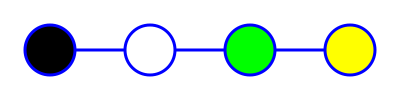
\includegraphics[width=0.6\textwidth]{img/graph/g08b.png}
		\end{center}
	\end{textblock*}

	\vspace{350px}

	\structure{出力}
	クラスを予測する分類森 $F$ \\
	\begin{textblock*}{0.45\textwidth}(0.6\hsize,-80pt)
		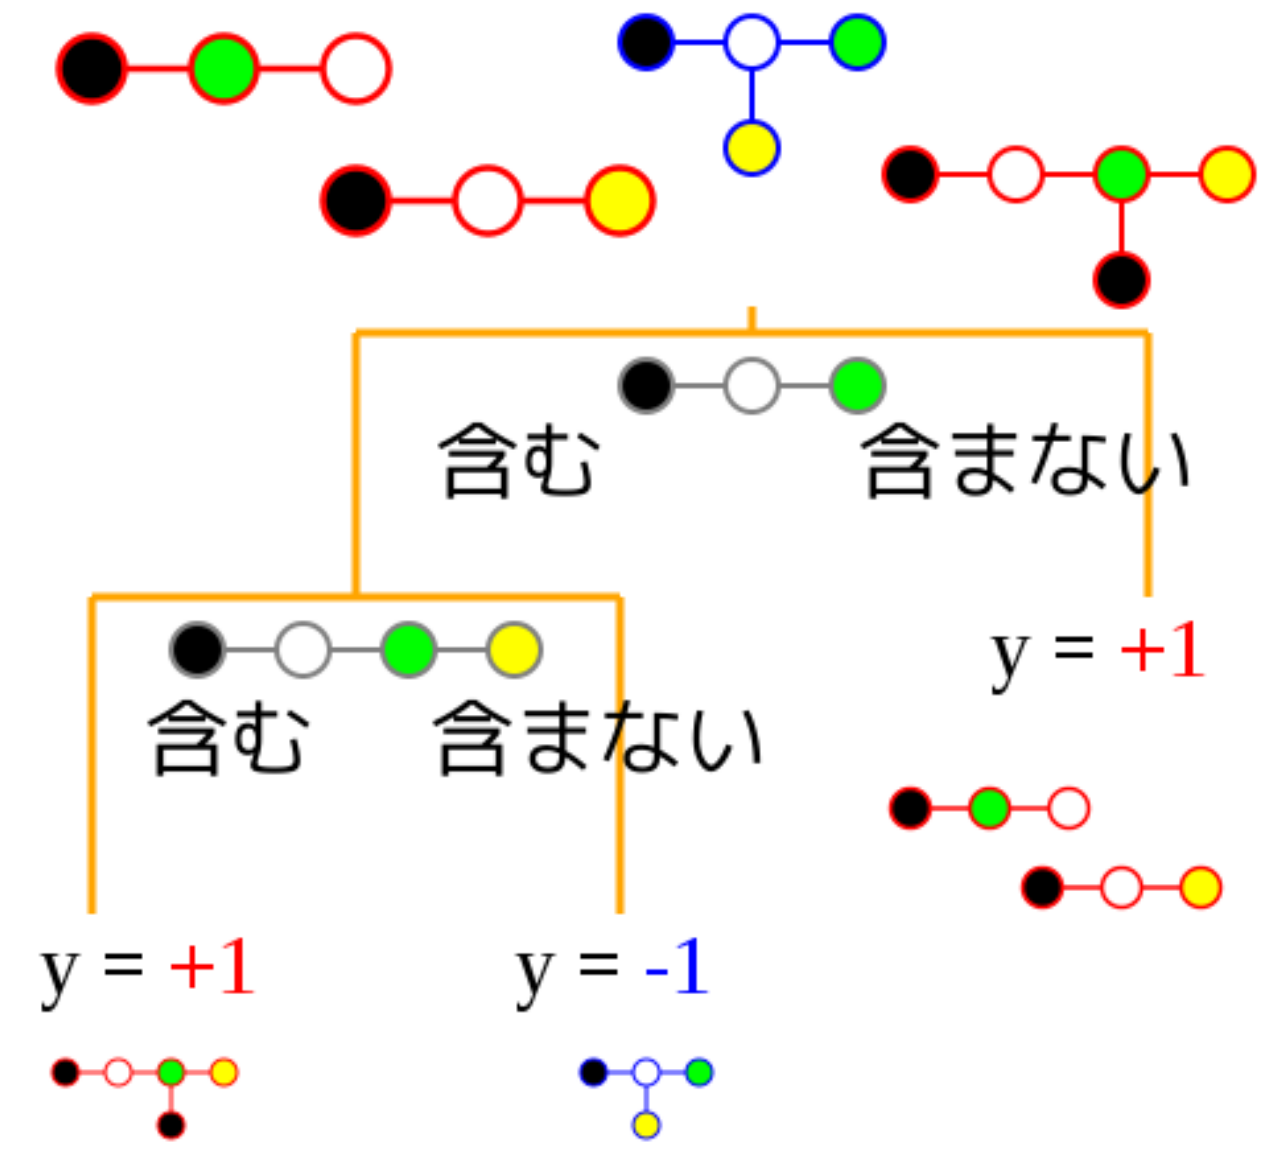
\includegraphics[width=0.8\textwidth]{img/dt.png}
	\end{textblock*}
	\begin{minipage}[t]{0.45\hsize}
		\begin{center}
			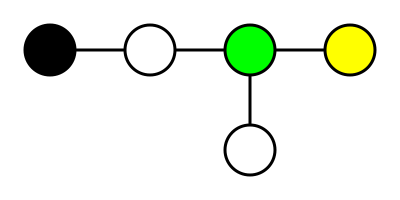
\includegraphics[width=0.24\textwidth]{img/graph/g09.png}
			\raisebox{30px}{$ \Rightarrow F \Rightarrow \plus \mbox{~or~} \minus $} \\
			\[
				F_t(x) = \sum_{i=1}^{t} f_i(x) = \sum_{i=1}^{t} \sum_{v \in \mbox{\footnotesize leaves of }f_i} w_v r_v
			\]
		\end{center}
	\end{minipage} \\
	\vspace{50pt}

	\structure{特徴ベクトル} 部分グラフの有無
	\begin{table}
		\begin{tabular}[b]{l|ccccr}
			&	
			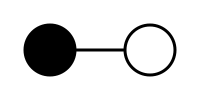
\includegraphics[width=0.1\textwidth]{img/subgraph/kw.png} &
			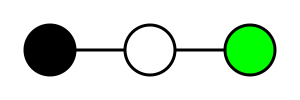
\includegraphics[width=0.1\textwidth]{img/subgraph/kwg.png} &
			\raisebox{10px}{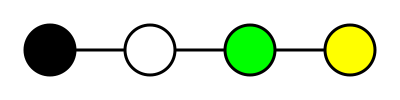
\includegraphics[width=0.1\textwidth]{img/subgraph/kwgy.png}} &
			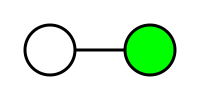
\includegraphics[width=0.1\textwidth]{img/subgraph/wg.png} &
			\raisebox{30px}{$\dots$} \\
			\hline
			\hline
			\raisebox{-.3\height}{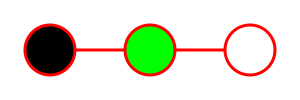
\includegraphics[width=0.12\textwidth]{img/graph/g01r.png}}	& 0 & 0 & 0 & 1 & \\
			\raisebox{-.3\height}{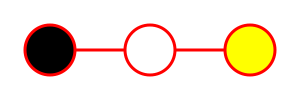
\includegraphics[width=0.12\textwidth]{img/graph/g03r.png}}	& 1 & 0 & 0 & 0 & \\
			\raisebox{-.5\height}{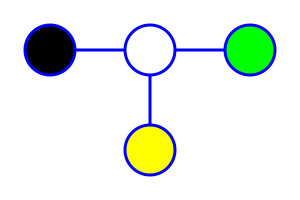
\includegraphics[width=0.12\textwidth]{img/graph/g05b.png}}	& 1 & 1 & 0 & 1 & \\
			\raisebox{-.5\height}{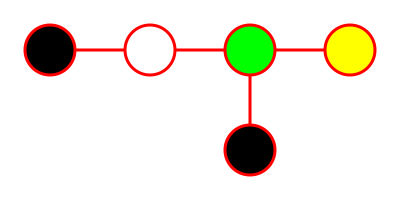
\includegraphics[width=0.12\textwidth]{img/graph/g07r.png}}	& 1 & 1 & 1 & 1 & \\
		\end{tabular}
	\end{table}
	\begin{tcolorbox}[colframe=white,colback=white,left=30px]
		全ての部分グラフに関して有無を調べるのは困難 \\
		頻出する部分グラフのみ調べる方法もあるが、 \\
		\alert{可能なら全ての部分グラフを活用したい!} \\
		GBDT なら可能だが精度が悪い。XGBoost, RGF でもしたい。
	\end{tcolorbox}
\end{tcolorbox}

		\begin{tcolorbox}[title={\Large Gradient~Boosting~Decition~Tree}]
	決定木を勾配ブースティングする。正則化を明示的に考えない。 \\
	決定木の大きさや縮小率を調整することで暗に正則化している。 \\
	明示的な正則化のなければ、全部分グラフ指示子に基づいて学習できる。 \\
	\[
		\min Q
		= \sum^N_{i=1} \Phi(y_i, F_t(x_i)) 
		= \sum^N_{i=1} \Phi(y_i, F_{t-1} + f_t) 
		\approx \sum^N_{i=1} \Phi(\tilde{y}^{(t-1)}_i, f_t) 
	\]
	\rightline{$ \tilde{y}^{(t-1)}_i = - \partial \Phi (y_i,F_{t-t}(x_i)) ~ / ~ \partial F_{t_1}(x_i) $} 


	\structure{全部分グラフ指示子に基づいた学習} \\
	\raisebox{-10pt}{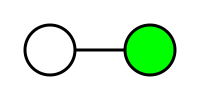
\includegraphics[height=\baselineskip]{img/subgraph/wg.png}}を \\
	\vspace{-60px}
	\begin{columns}[t]
		\begin{column}{0.50\hsize}
			\begin{tcolorbox}[colback=white]
				含まない \\
				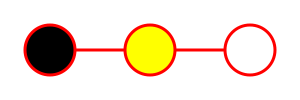
\includegraphics[height=1\baselineskip]{img/graph/g02r.png} \hspace{30px}
				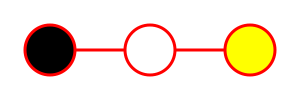
\includegraphics[height=1\baselineskip]{img/graph/g03r.png} \\
				\vspace{10px} \\
				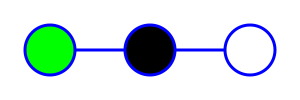
\includegraphics[height=1\baselineskip]{img/graph/g04b.png} \\
			\end{tcolorbox}
		\end{column}
		\begin{column}{0.50\hsize}
			\begin{tcolorbox}[colback=white]
				含む \\
				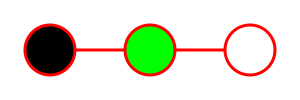
\includegraphics[height=1\baselineskip]{img/graph/g01r.png} \hspace{30px}
				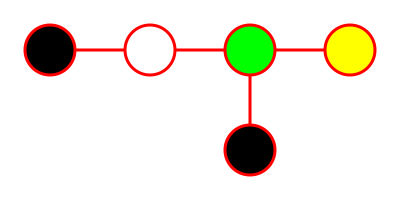
\includegraphics[height=2\baselineskip]{img/graph/g07r.png} \\
				\vspace{10px} \\
				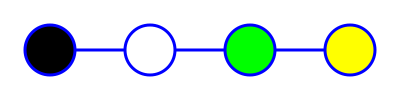
\includegraphics[height=1\baselineskip]{img/graph/g08b.png}
				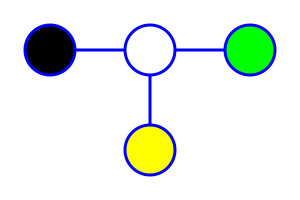
\includegraphics[height=2\baselineskip]{img/graph/g05b.png}
				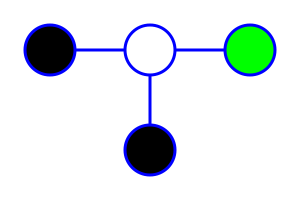
\includegraphics[height=2\baselineskip]{img/graph/g06b.png}
			\end{tcolorbox}
		\end{column}
	\end{columns}

	\vspace{60px}
	ここまで分かっているとき、 \\
	\raisebox{-10pt}{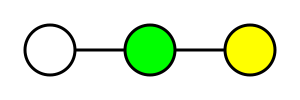
\includegraphics[height=\baselineskip]{img/subgraph/wgy.png}}の有無で分割することを考える \\

	理想の分割($\plus$のみ含む) \\
	\vspace{-60px}
	\begin{columns}[t]
		\begin{column}{0.50\hsize}
		\begin{tcolorbox}[colback=white]
			含まない \\
			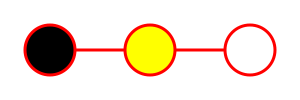
\includegraphics[height=0.7\baselineskip]{img/graph/g02r.png} \hspace{30px}
			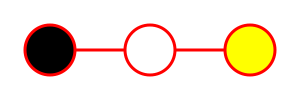
\includegraphics[height=0.7\baselineskip]{img/graph/g03r.png} \\
			\vspace{10px} \\
			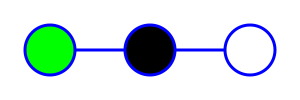
\includegraphics[height=0.7\baselineskip]{img/graph/g04b.png} \hspace{10px}
			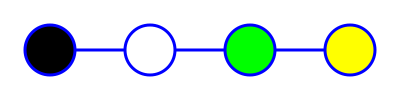
\includegraphics[height=0.7\baselineskip]{img/graph/g08b.png} \hspace{10px}
			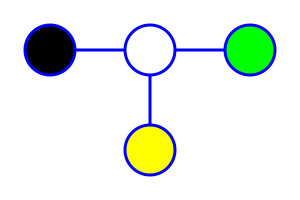
\includegraphics[height=1.4\baselineskip]{img/graph/g05b.png} \hspace{10px}
			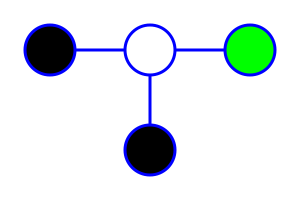
\includegraphics[height=1.4\baselineskip]{img/graph/g06b.png}
		\end{tcolorbox}
		\end{column}
		\begin{column}{0.50\hsize}
		\begin{tcolorbox}[colback=white,colframe=red]
			含む \\
			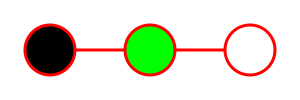
\includegraphics[height=0.7\baselineskip]{img/graph/g01r.png} \hspace{30px}
			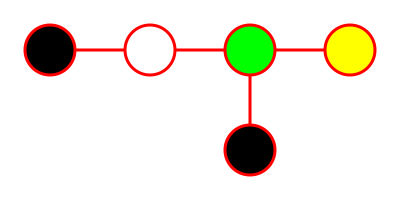
\includegraphics[height=1.4\baselineskip]{img/graph/g07r.png} \\
		\end{tcolorbox}
		\end{column}
	\end{columns}

	\vspace{50px}

	理想の分割($\minus$のみ含む) \\
	\vspace{-60px}
	\begin{columns}[t]
		\begin{column}{0.50\hsize}
		\begin{tcolorbox}[colback=white]
			含まない \\
			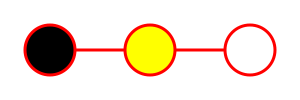
\includegraphics[height=0.7\baselineskip]{img/graph/g02r.png} \hspace{30px}
			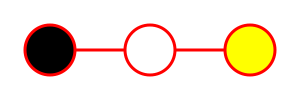
\includegraphics[height=0.7\baselineskip]{img/graph/g03r.png} \\
			\vspace{10px} \\
			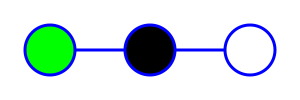
\includegraphics[height=0.7\baselineskip]{img/graph/g04b.png} \hspace{30px}
			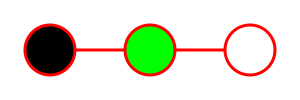
\includegraphics[height=0.7\baselineskip]{img/graph/g01r.png} \hspace{30px}
			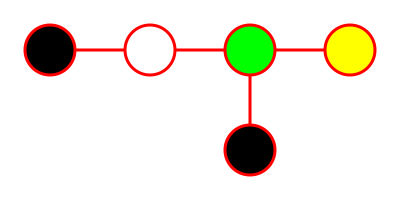
\includegraphics[height=1.4\baselineskip]{img/graph/g07r.png} \\
		\end{tcolorbox}
		\end{column}
		\begin{column}{0.50\hsize}
		\begin{tcolorbox}[colback=white,colframe=blue]
			含む \\
			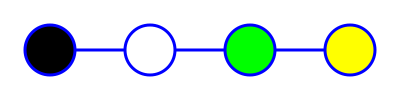
\includegraphics[height=0.7\baselineskip]{img/graph/g08b.png}
			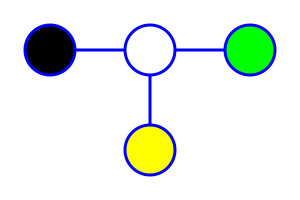
\includegraphics[height=1.4\baselineskip]{img/graph/g05b.png}
			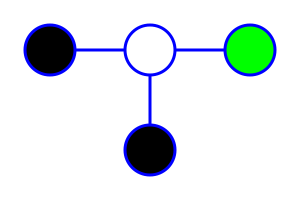
\includegraphics[height=1.4\baselineskip]{img/graph/g06b.png}
		\end{tcolorbox}
		\end{column}
	\end{columns}



\end{tcolorbox}

	\end{column}
	\begin{column}{0.50\hsize}
		\begin{tcolorbox}[title={\Large XGBoost}]
	パッケージ化されており、並列処理などによる高速化がされている。 \\
	明示的な正則化があり、目的関数の近似にヘシアンも使う。 \\
	\color{ash}
	\begin{eqnarray*}
		\min Q
		&=& \sum^N_{i=1} \Phi(y_i, F_t(x_i)) + \Omega(F_t)
		= \sum^N_{i=1} \Phi(y_i, F_{t-1} + f_t) + \Omega(f_t)  \\
		&\approx& \sum^N_{i=1} [ \Phi(\tilde{y}^{(t-1)}_i, y_i) +g_if_t(x_i) + \frac{1}{2}h_if_t^{\large 2}(x_i) ] +\Omega(f_t) \\
		&=& \sum^N_{i=1} [ g_if_t(x_i) + \frac{1}{2}h_if_t^{\large 2}(x_i) ] +
		\gamma T + \frac{1}{2} \lambda \sum^T_{j=1} w_j^2 \\
		&=& \sum_{v \in \mbox{\footnotesize leaves of }f_i} [ (\sum_{i \in r_v} g_i) w_j + \frac{1}{2} (\sum_{i \in r_v}h_i + \lambda) w_j^2 ]
		+ \gamma T \\
	\end{eqnarray*}

	\hspace{600px}
	\begin{minipage}[t]{0.45\hsize}
		$ \hat{y_i}^{(t-1)}  = F_{t_1}(x_i) $ \\
		$ g_i  = \partial_{\hat{y}^(t-1)} \Phi(y_i, \hat{y_i}^{(t-1)}) $ \\
		$ h_i  = \partial^2_{\hat{y}^(t-1)} \Phi(y_i, \hat{y_i}^{(t-1)}) $ \\
		$ \Omega(f_t) = \gamma T + \frac{1}{2} \lambda \sum^T_{j=1} w_j^2 $ \\
		$T$ は $f_t$ の葉ノードの数 \\
	\end{minipage}

	$f_t$ を固定すると、最適な$w^\ast$が計算できる。
	\[ w^\ast_j = - \frac{\sum_{i \in r_v}g_i}{\sum_{i \in r_v}h_i + \lambda} \]

	このとき、目的関数は
	\[
		\tilde{Q}(f_t) = - \frac{1}{2} \sum_{v \in \mbox{\footnotesize leaves of }f_i}
		\frac{(\sum_{i \in r_v}g_i)^2}{\sum_{i \in r_v}h_i + \lambda} + \gamma T
	\]
	$f_t$ の $r_0$ を $r_1$ と $r_2$ に分割するときの目的関数の差分は
	\[
		\frac{1}{2} [
			\frac{(\sum_{i \in r_1}g_i)^2}{\sum_{i \in r_1}h_i + \lambda}
			+ \frac{(\sum_{i \in r_2}g_i)^2}{\sum_{i \in r_2}h_i + \lambda}
			- \frac{(\sum_{i \in r_0}g_i)^2}{\sum_{i \in r_0}h_i + \lambda}
		] - \gamma
	\]

	\color{black}
	\normalsize
	分割の目的は
	\[
		\min \Biggl[
			\frac{(\sum_{i \in r_1}g_i)^2}{\sum_{i \in r_1}h_i + \lambda}
			+ \frac{(\sum_{i \in r_2}g_i)^2}{\sum_{i \in r_2}h_i + \lambda}
		\Biggr]
	\]

	\begin{textblock*}{\textwidth}(0.78\hsize,-230pt)
			\begin{tabular}{ccc}
				\raisebox{-.3\height}{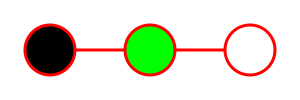
\includegraphics[width=0.12\textwidth]{img/graph/g01r.png}}	& $g_1$ & $h_1$ \\
				\raisebox{-.3\height}{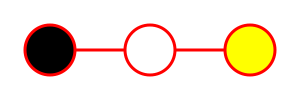
\includegraphics[width=0.12\textwidth]{img/graph/g03r.png}}	& $g_2$ & $h_2$ \\
				\raisebox{-.5\height}{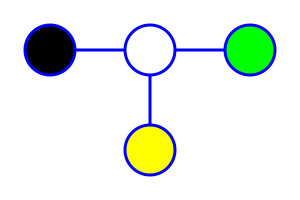
\includegraphics[width=0.12\textwidth]{img/graph/g05b.png}}	& $g_3$ & $h_3$ \\
				\raisebox{-.5\height}{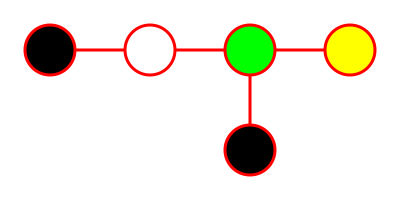
\includegraphics[width=0.12\textwidth]{img/graph/g07r.png}}	& $g_4$ & $h_4$ \\
			\end{tabular}
	\end{textblock*}



\end{tcolorbox}

		\begin{tcolorbox}[title={\Large Regularized Greedy Forest}]
	定期的に、全ての葉の重みを計算しなおすことで \\
	収束を早め、簡潔なモデルを作成する。 \\
	明示的な正則化があり、勾配ブースティングよりも調整しやすい。 \\
	決定木単位ではなく、葉ノード単位でアンサンブルを行う。 \\

	\begin{columns}
		\begin{column}{0.50\hsize}
			\[ F(x_i) = \sum_{v \in \mbox{\footnotesize leaves of }F} w_v r_v \]

			\vspace{50px}
			$r_0$ を $r_1$ と $r_2$ に分割した分類森 $F'$ は
			\begin{eqnarray*}
				F'
				&=& F - w_0 r_0 + w_1 r_1 + w_2 r_2  \\
				&=& F - w_0 r_0 + (w_0 + \delta_1) r_1 + (w_0 + \delta_1) r_2  \\
				&=& F + \delta_1 r_1 + \delta_2 r_2  \\
			\end{eqnarray*}

			\vspace{-70px}
			\[ \hat{\delta}_k = - \frac{Q'(F(\delta_1, \delta_2))}{Q''(F'(\delta_1, \delta_2))} \mid_{\delta_1=0, \delta_2=0} \]

		\end{column}
		\begin{column}{0.50\hsize}
			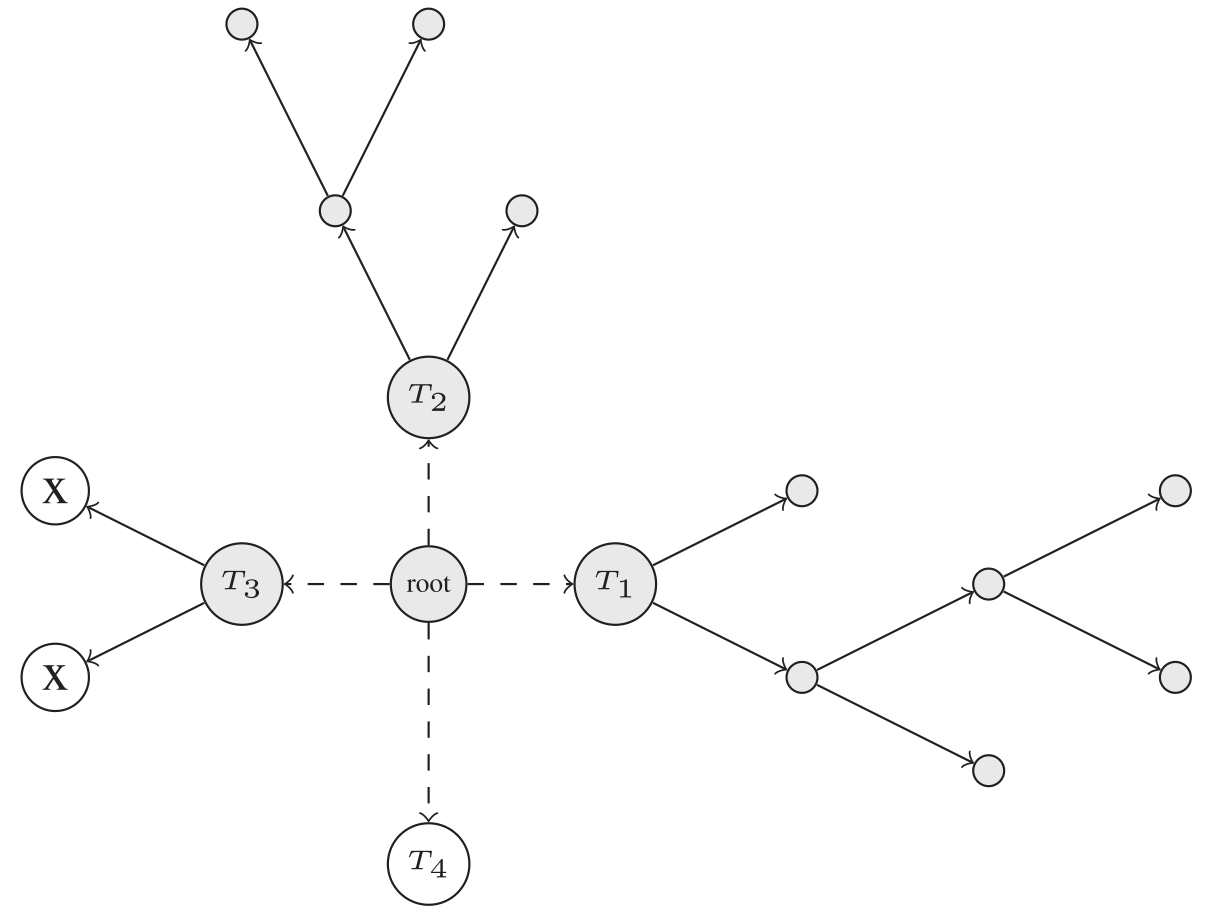
\includegraphics[width=1.0\textwidth]{img/rgf.png}
			\begin{textblock*}{\textwidth}(450pt,0pt)
				{\footnotesize 出典\cite{rgf}}
			\end{textblock*}
		\end{column}
	\end{columns}

	\vspace{40px}
	目的関数 $Q$ は
	\[
		\min Q
		= \sum^N_{i=1} \Phi(y_i, F(x_i)) + \Omega(F)
		= \sum^N_{i=1} \Phi(y_i, F(x_i)) + \lambda \sum_v w_v^2 / 2
	\]
	分割の目的は
	\begin{eqnarray*}
		\min Q' - Q
		&=& \Phi(y_i, w_1 r_1) + \Phi(y_i, w_2 r_2) - \Phi(y_i, w_0 r_0) + w_1^2 + w_2^2 - w_0^2 \\
		&=& \Phi(y_i, w_1 r_1) + \Phi(y_i, w_2 r_2) + w_1^2 + w_2^2 \\
	\end{eqnarray*}

\end{tcolorbox}

		\begin{tcolorbox}[title={\Large 参考文献}]
	\begin{thebibliography}{99}
			\beamertemplatetextbibitems
		\bibitem{gbdt} Friedman, Jerome H. "Stochastic Gradient Boosting." mh (x; am) 1000 (1999): 0.
		\bibitem{xgboost} Chen, Tianqi, and Carlos Guestrin. "Xgboost: A scalable tree boosting system." arXiv preprint arXiv:1603.02754 (2016).
		\bibitem{rgf} Johnson, Rie, and Tong Zhang. "Learning nonlinear functions using regularized greedy forest." IEEE transactions on pattern analysis and machine intelligence 36.5 (2014): 942-954.
	\end{thebibliography}
\end{tcolorbox}

	\end{column}
\end{columns}

\end{document}
